\chapterimage{img/inv.jpg} 
\chapter{Inverse Functions}
\section{Inverse Functions}
Recall that a function can be represented by a set of ordered pairs. For instance, the function $f(x)=x+4$ from the set $A ={1, 2, 3, 4}$ to the set $B = {5, 6, 7, 8}$ can be written as follows. \cite{ci}
$$f(x) = x+4: {(1,5),(2,6),(3,7),(4,8)}$$
In this case, by interchanging the first and second coordinates of each of these ordered pairs, you can form the \textbf{inverse function} of $f$, which is denoted by $f^{-1}$. It is a function from the set $B$ to the set $A$, and can be written as follows. \cite{ci}
$$f^{-1}(x) = x-4: {(5,1),(6,2),(7,3),(8,4)}$$
Note that the domain of $f$ is equal to the range of $f^{-1}$, and vice versa, as shown in Figure \ref{fig:domain_inv}. Also note that the functions $f$ and $f^{-1}$ have the effect of “undoing” each other. In other words, when you form the composition of $f$ with $f^{-1}$ or the composition of $f^{-1}$ with $f$, you obtain the identity function. \cite{ci}

$$f(f^{-1}(x))=f(x-4)=(x-4)+4=x$$
$$f^{-1}(f(x))=f^{-1}(x+4)=(x+4)-4=x$$

\begin{figure}[H]
    \centering
    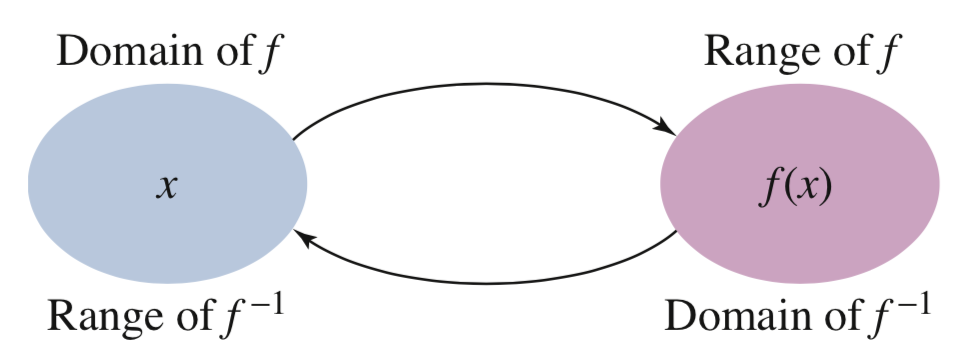
\includegraphics[scale=0.5]{img/fig/domain_inv.png}
    \caption{Domain of an Inverse Function \cite{ci}}
    \label{fig:domain_inv}
\end{figure}

\begin{definition}
    Let $f$ and $g$ be two functions such that
    $$f(g(x))=x\qquad \text{for every $x$ in the domain of $g$}$$
    and
    $$g(f(x))=x\qquad \text{for every $x$ in the domain of $f$}$$
    Under these conditions, the function $g$ is the \textbf{inverse function} of the function $f$. The function $g$ is denoted by $f^{-1}$ (read “f-inverse”). 
    \\\cite{ci}
\end{definition}

If the function $g$ is the inverse function of the function $f$, it must also be true that the function $f$ is the inverse function of the function $g$. For this reason, you can say that the functions $f$ and $g$ are \textit{inverse functions of each other}.

\section{The Graph of an Inverse Function}
The graphs of a function $f$ and its inverse function $f^{-1}$ are related to each other in the following way. If the point $(a,b)$ lies on the graph of $f$, then the point $(b,a)$ must lie on the graph of $f^{-1}$, and vice versa. This means that the graph of $f^{-1}$ is a reflection of the graph of $f$ in the line $y = x$, as shown in Figure \ref{plot:inv func}.

\begin{figure}[H]
    \centering
    \begin{tikzpicture}
        \begin{axis}[
                nejes=-3:3 -3:3,xlabel=$x$, ylabel=$y$
            ]
            \addplot [very thick, penColor, smooth] {x^3} node[pos=0.7, above left, black] {$f(x)$};
            \addplot [very thick, penColor2, smooth] {x/abs(x)*abs(x)^(1/3)} node[pos=0.8, below right, black] {$f^{-1}(x)$};
            \draw[dashed, black, thick] (axis cs:-3,-3) -- (axis cs:3,3);
            \draw[dashed, black, thick] (axis cs:-2,-1.2599210499) -- (axis cs:-1.2599210499,-2);
            \addplot [soldot, black] coordinates{(-2,-1.2599210499)} node[pos=-0.2, above left,black] {$(b,a)$};
            \addplot [soldot, black] coordinates{(-1.2599210499,-2)} node[pos=-0.2, below right,black] {$(a,b)$};
        \end{axis}
    \end{tikzpicture}
    \caption{A plot of a pair of Inverse Functions.}
    \label{plot:inv func}
\end{figure}


\section{Finding Inverse Functions Analytically}
For simple functions, you can find inverse functions by inspection. For more complicated functions, however, it is best to use the following guidelines. The key step in these guidelines is Step 3—interchanging the roles of $x$ and $y$. This step corresponds to the fact that inverse functions have ordered pairs with the coordinates reversed. \cite{ci}

\begin{proposition}[Guidelines For Finding Inverse Functions]\cite{ci}
    ~\\
    \begin{enumerate}
        \item Use the Horizontal Line Test to decide whether $f$ has an inverse function.
        \item In the equation for $f(x)$, replace $f(x)$ by $y$.
        \item Interchange the roles of $x$ and $y$, and solve for $y$.
        \item Replace $y$ by $f^{-1}(x)$ in the new equation.
    \end{enumerate}
\end{proposition}
~\\
\begin{example}[Finding an Inverse Function Analytically] \cite{ci}~\newline
    Find the inverse function of $f(x)=\dfrac{5-3x}{2}.$\\
    \begin{solution}~\newline
        Since $f(x)$ is a linear function, the graph of $f$ is a line which passes the Horizontal Line Test. So, you know that $f$ is one-to-one and has an inverse function.
        \begin{align*}
            f(x)&=\dfrac{5-3x}{2}&&\text{Write original function.}\\
            y&=\dfrac{5-3x}{2}&&\text{Replace $f(x)$ by $y$.}\\
            x&=\dfrac{5-3y}{2}&&\text{Interchange $x$ and $y$.}\\
            2x&=5-3y&&\text{Multiply each side by 2.}\\
            3y&=5-2x&&\text{Isolate the $y$-term.}\\
            y&=\dfrac{5-2x}{3}&&\text{Solve for $y$.}\\
            f^{-1}(x)&=\dfrac{5-2x}{3}&&\text{Replace $y$ by $f^{-1}(x)$.}\\
        \end{align*}
        Note that both $f$ and $f^{-1}$ have domains and ranges that consist of the entire set of real numbers.
	\end{solution}
\end{example}

\begin{example}[Finding an Inverse Function Analytically] \cite{ci}~\newline
    Find the inverse function of $f(x)=\sqrt{2x-3}.$\\
    \begin{solution}~\newline
        The graph of $f$ is a curve, as shown in Figure \ref{plot:sqrt2x-3}. Because this graph passes the Horizontal Line Test, you know that $f$ is one-to-one and has an inverse function.
        \begin{figure}[H]
            \centering
            \begin{tikzpicture}
                \begin{axis}[
                        nejes=-3:6 -2:5,xlabel=$x$, ylabel=$y$
                    ]
                    \addplot [very thick, penColor, smooth, samples at={1.50,1.51,...,1.55,...,2.5,3,...,6}] {sqrt(2*x-3)} node[pos=0.9, above left, black] {$f^{-1}(x)$};
                    \addplot [domain=0:5, very thick, penColor2, smooth] {(x^2+3)/2)} node[pos=0.4, below right, black] {$f(x)$};
                    \draw[dashed, black, thick] (axis cs:-2,-2) -- (axis cs:5,5);
                    \addplot [soldot, black] coordinates{(0,1.5)} node[pos=-0.2, above left,black] {$(0,1.5)$};
                    \addplot [soldot, black] coordinates{(1.5,0)} node[pos=-0.2, below right,black] {$(1.5,0)$};
                    \addplot [noldot] coordinates{(-2,-2)} ;
                \end{axis}
            \end{tikzpicture}
            \caption{A plot of $\sqrt{2x-3}$.}
            \label{plot:sqrt2x-3}
        \end{figure}
        \begin{align*}
            f(x)&=\sqrt{2x-3}&&\text{Write original function.}\\
            y&=\sqrt{2x-3}&&\text{Replace $f(x)$ by $y$.}\\
            x&=\sqrt{2y-3}&&\text{Interchange $x$ and $y$.}\\
            x^2&=2y-3&&\text{Square each side.}\\
            2y&=x^2+3&&\text{Isolate $y$.}\\
            y&=\dfrac{x^2+3}{2}&&\text{Solve for $y$.}\\
            f^{-1}(x)&=\dfrac{x^2+3}{2}&&\text{Replace $y$ by $f^{-1}(x)$.}\\
        \end{align*}
        The graph of $f^{-1}$ in Figure \ref{plot:sqrt2x-3} is the reflection of the graph of $f$ in the line $y=x$. Note that the range of $f$ is the interval $[0,\infty)$, which implies that the domain of $f^{-1}$ is the interval $[0,\infty)$. Moreover, the domain of $f$ is the interval $\left[\dfrac{2}{3},\infty\right)$, which implies that the range of $f^{-1}$ is the interval $\left[\dfrac{2}{3},\infty\right)$.
	\end{solution}
\end{example}

\begin{exercise}
    ~\\\-\hspace{0.3cm} \textbf{
        In Exercises 1–3, show that $f$ and $g$ are inverse functions analytically.
    }\cite{ci}\\
    \begin{enumerate} 
		\item $f(x) = 2x,\quad g(x)=\dfrac{x}{2}$
		\item $f(x) = \dfrac{1}{x},\quad g(x)=\dfrac{1}{x}$
    \end{enumerate}
    ~\\\-\hspace{0.3cm} \textbf{
        In Exercises 3–6, determine whether the function has an inverse function. If it does, find the inverse function.
    }\cite{ci}\\
    \begin{enumerate}
        \setcounter{enumi}{2}
        \item $f(x) = \dfrac{x}{8}$
        \item $f(x) = -4$
        \item $f(x) = \sqrt{2x+3}$
        \item $h(x) = -\dfrac{4}{x^2}$
    \end{enumerate}
\end{exercise}
